\documentclass{amsart}
\synctex=1

%=================================================================
% 
\newcount\DraftStatus  % 0 suppresses notes to selves in text
\DraftStatus=1   % TODO: set to 0 for final version
%=================================================================

%=================================================================
\usepackage{comment}
%=================================================================
%
\includecomment{JournalOnly}  
\includecomment{ConferenceOnly}  
\includecomment{TulipStyle}
%
%=================================================================
\input{preamble}


%=================================================================
%
\begin{document}
%
%=================================================================
%
\title[A Short Running Title]{Kaggle Report}%

\author{Huanhuan Ge}
\address[A.~1]{School of Computer Science,\\ 
Qingdao University of Technology, Qingdao, China}%
\email[A.~1]{18852862723@163.com}

% \author{Gang Li}
% \address[A.~2]{School of Information Technology \\
% Deakin University, Geelong, VIC 3216, Australia}%
% \email[A.~2]{gang.li@deakin.edu.au}

% \author{Author 3}
% \address[A.~3]{School of Information Technology \\
% Deakin University \\
% Vic 3125, Australia}%
% \email[A.~3]{xxx@deakin.edu.au}

%\thanks{Thanks to \ldots}%
\subjclass{Artificial Intelligence}%
\date{\gitAuthorDate}%


\begin{abstract}
In this report,I will talk about my Kaggle Project.In previous studies, I learned the use of Latex and Git and mastered their basic operations.  I also learned about Python and data visualization. 
Now I'm going to use the Kaggle project to demonstrate what I've learned.
\end{abstract}

\keywords{Python,Machine Learning, Data Processing,Git,Latex}%




\maketitle
\tableofcontents

\newpage
%=================================================================

%=================================================================
\section{Introduction}\label{sec-intro}

\subsection{Description}
In a world… where movies made an estimated \$41.7 billion in 2018, the film industry is more popular than ever. 
But what movies make the most money at the box office? How much does a director matter? Or the budget? For some movies, 
it's "You had me at 'Hello.'" For others, the trailer falls short of expectations and you think "What we have here is a
failure to communicate." 
\subsection{Target}
In this competition, you're presented with metadata on over 7,000 past films from The Movie Database to try and predict 
their overall worldwide box office revenue. Data points provided include cast, crew, plot keywords, budget, posters,
 release dates, languages, production companies, and countries. You can collect other publicly available data to use 
 in your model predictions, but in the spirit of this competition, use only data that would have been available before 
 a movie's release. 

 \section{Data Processing} \label{sec-preliminaries}
 \subsection{Data Description}
 In the dataset, it includes 7,398 movies and various metadata from the Movie
Database (TMDB), Movies are labeled with id.Data points include cast,crew,plot keywords, budget, posters, release dates, 
languages, production companies, and countries.Predict the worldwide revenue for 4398 movies.

\subsection{Basic Information of Data}
\begin{itemize}
	\smallskip
	\item \textbf{train.csv} -- it contains 3000 rows and 23 columns.
	\smallskip
	\item \textbf{test.csv} -- it contains 4398 rows and 22 columns. Compared with the train data, there are fewer "revenue" column.
	\smallskip
	\item \textbf{sample\_submission.csv} -- it clarifies the data submission format. It just contains 2 columns that is "id" and "revenue".
\end{itemize}
\subsection{Data Fields}  
The following is basic information of data. \\
\begin{tabular}{p{3cm}p{2cm}p{7cm}}
  \toprule
  \centering
  Name
  & Description & Attribute \\
  \midrule
  \centering 
  train.csv
  & {Training set(Movies from $1970$-$2018$)} &  {id,belongs\_to\_collection,budget,genres,homepage,
  imdb\_id,original\_language,original\_title,overview,
  popularity,poster\_path,production\_companies,
  production\_countries,release\_date,runtime,
  spoken\_languages,status,tagline,title,Keywords,
  cast,crew,revenue}  \\
  \centering 
  test.csv
  & {Test set(Predict revenue)} &  {id,belongs\_to\_collection,budget,genres,homepage,
  imdb\_id,original\_language,original\_title,overview,
  popularity,poster\_path,production\_companies,
  production\_countries,release\_date,runtime,
  spoken\_languages,status,tagline,title,Keywords,
  cast,crew} \\
  \centering
  sample\_submission.csv &  {Format of submission} &  {id,revenue} \\
  \bottomrule
  \end{tabular}
  \subsection{Numerical features} 
  \begin{itemize}
    \item  There are $4$ numerical features in total.
    \smallskip
    \item  The minimum of budget is $0$.
    \smallskip
    \item There are some missing values in the runtime, and the minimum of runtime is $0$.
  \end{itemize}

  \begin{figure}[htbp]
    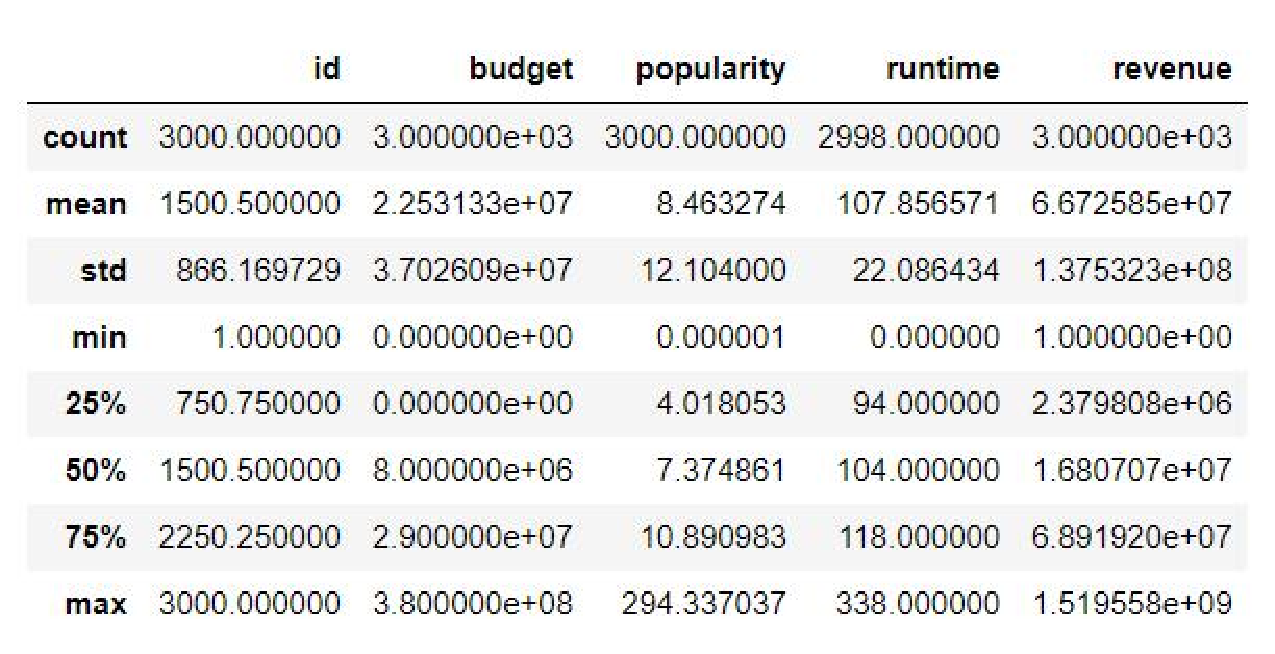
\includegraphics[scale=0.5]{./figures/describe.eps}
    \caption{Numerical features}
  \end{figure}


\subsection{Missing Value} 
Below is the missing field information. \\
\begin{figure}[htbp]
  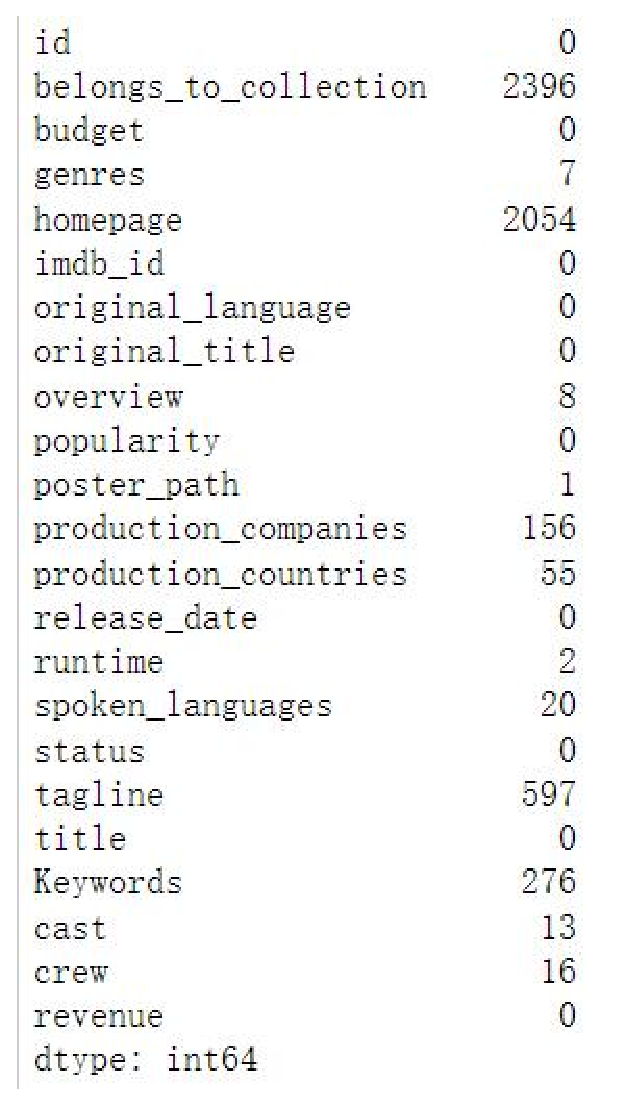
\includegraphics[scale=0.4]{./figures/MissingValue.eps}
  \caption{Missing values analysis}
\end{figure}
We're going to remove some characteristic dimensions,such as columns that contain many null-valued features,
columns from which Prediction of Revenue does not affect.



\subsection{Process Genres}
Genres contains all type names and TMDB ids in JSON format.
The type information in JSON format needs to be parsed. The following figure shows the parsing result. \\

\begin{figure}[htbp]
  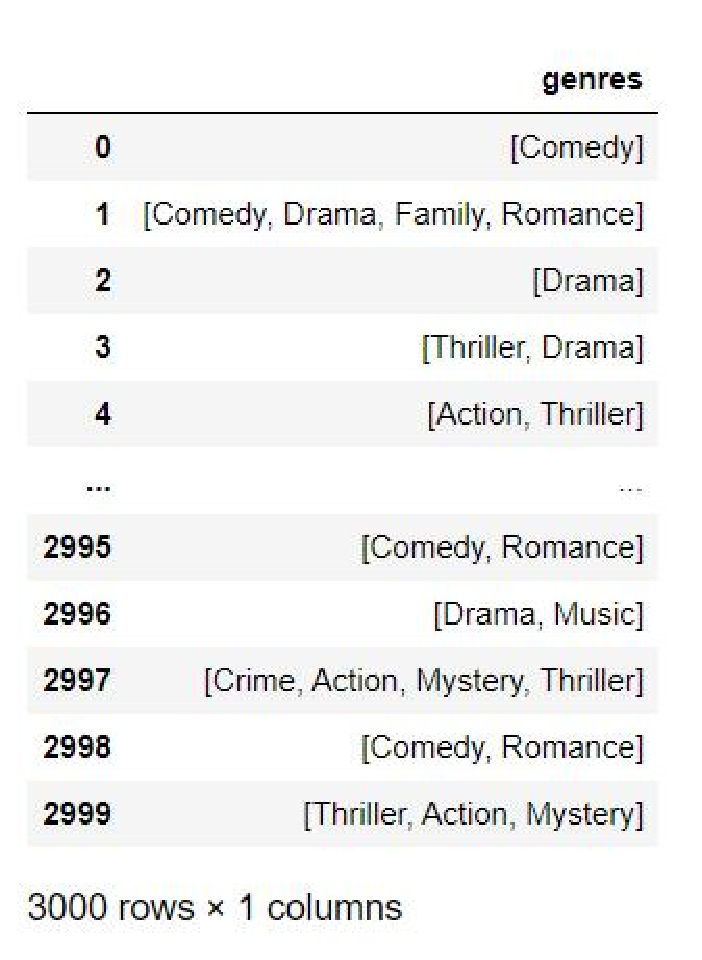
\includegraphics[scale=0.5]{./figures/genres.eps}
  \caption{Genres}
\end{figure}


\subsection{Release date}
The Date data of the Date type needs to be parsed into three dimensions: release year, release month, and release Date. 
The analysis result is shown in the following figure. \\

\begin{figure}[htbp]
  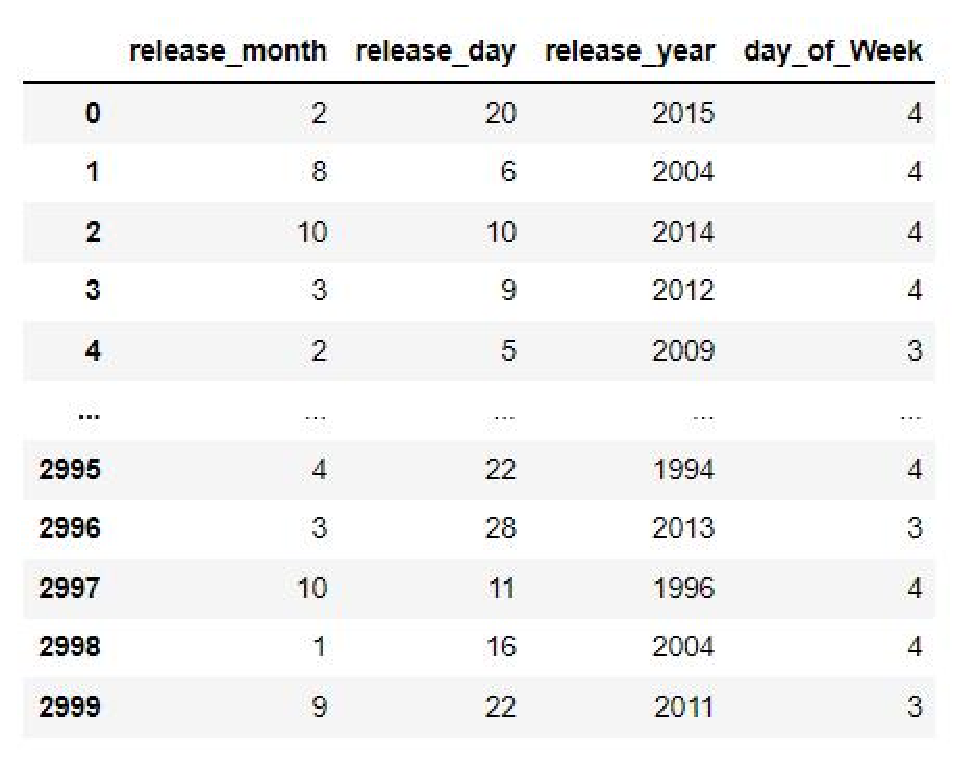
\includegraphics[scale=0.4]{./figures/date1.eps}
  \caption{Date}
\end{figure}



\subsection{Data visualization}
Next, I will make a visual analysis of the impact of budget, popularity, Genres,runtime and date on revenue.
 \\

\begin{figure}[htbp]
  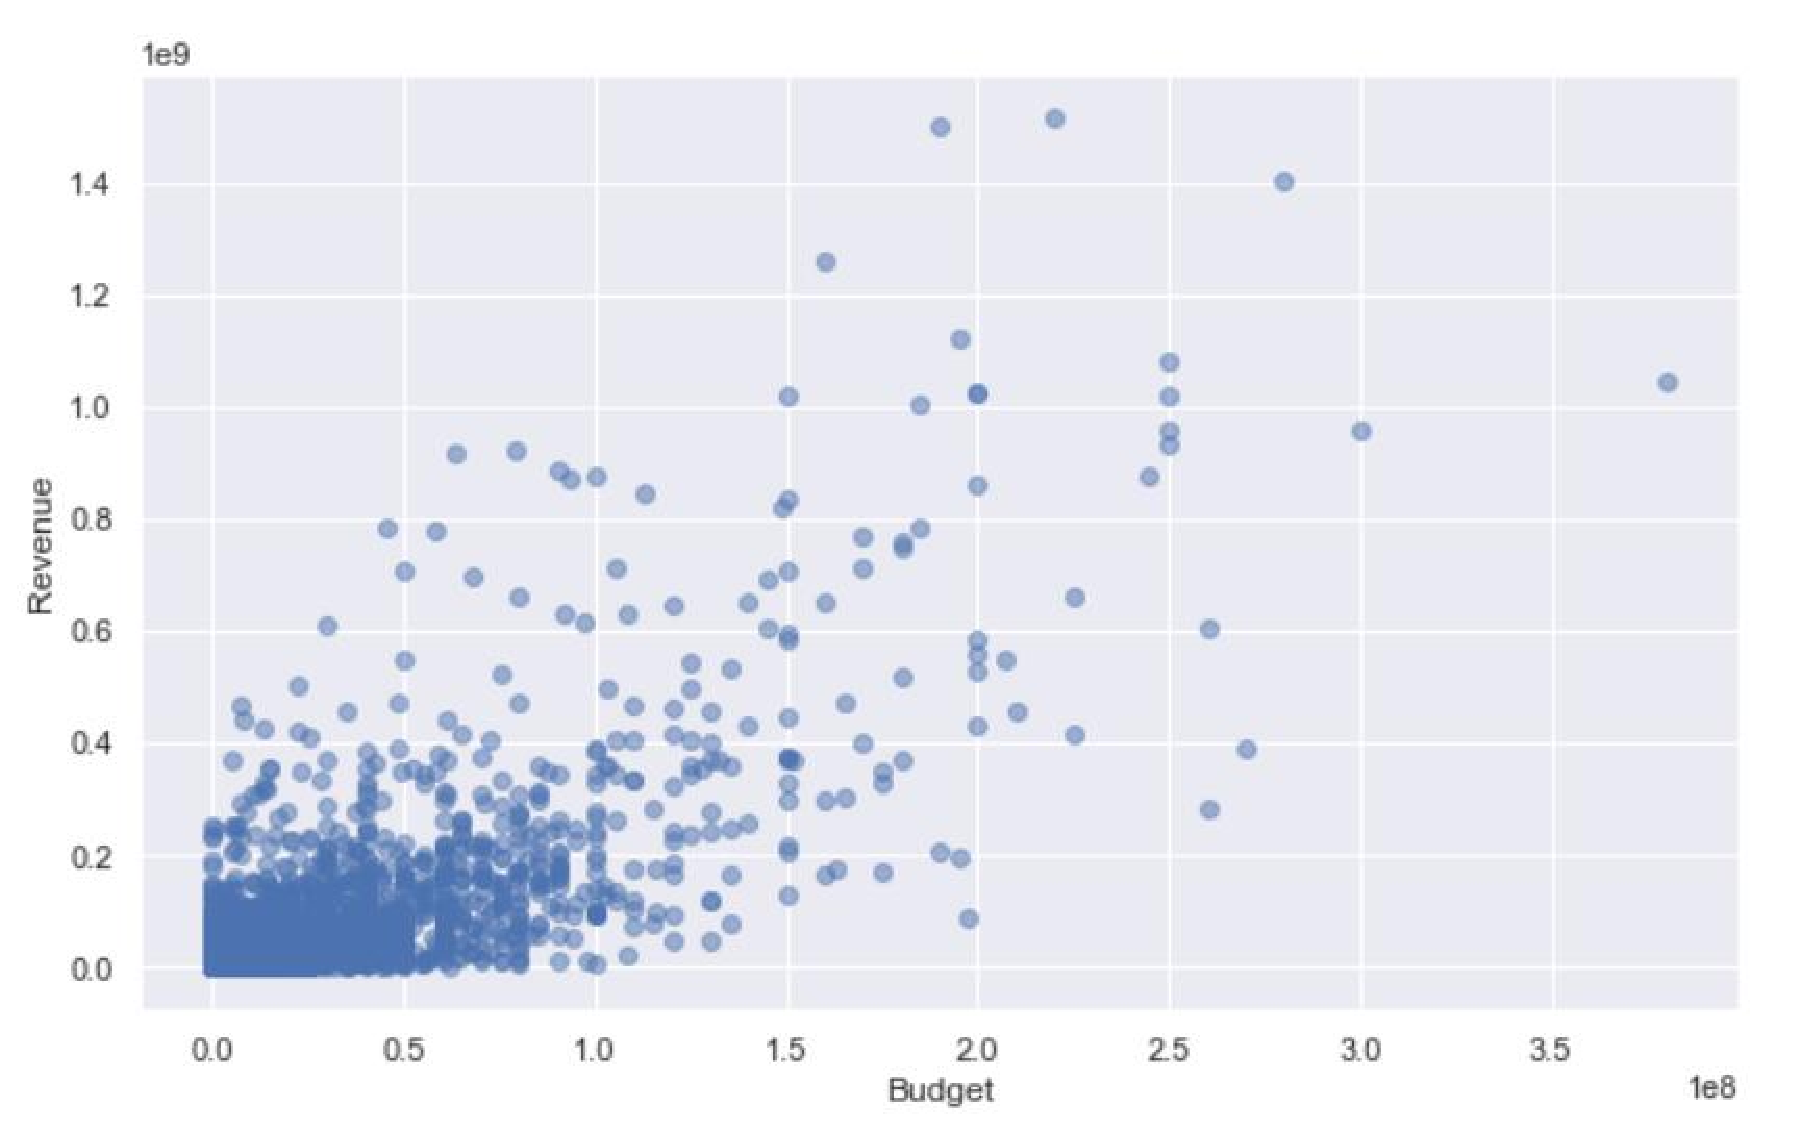
\includegraphics[scale=0.4]{./figures/budget2.eps}
  \caption{budget}
\end{figure}

\begin{figure}[htbp]
  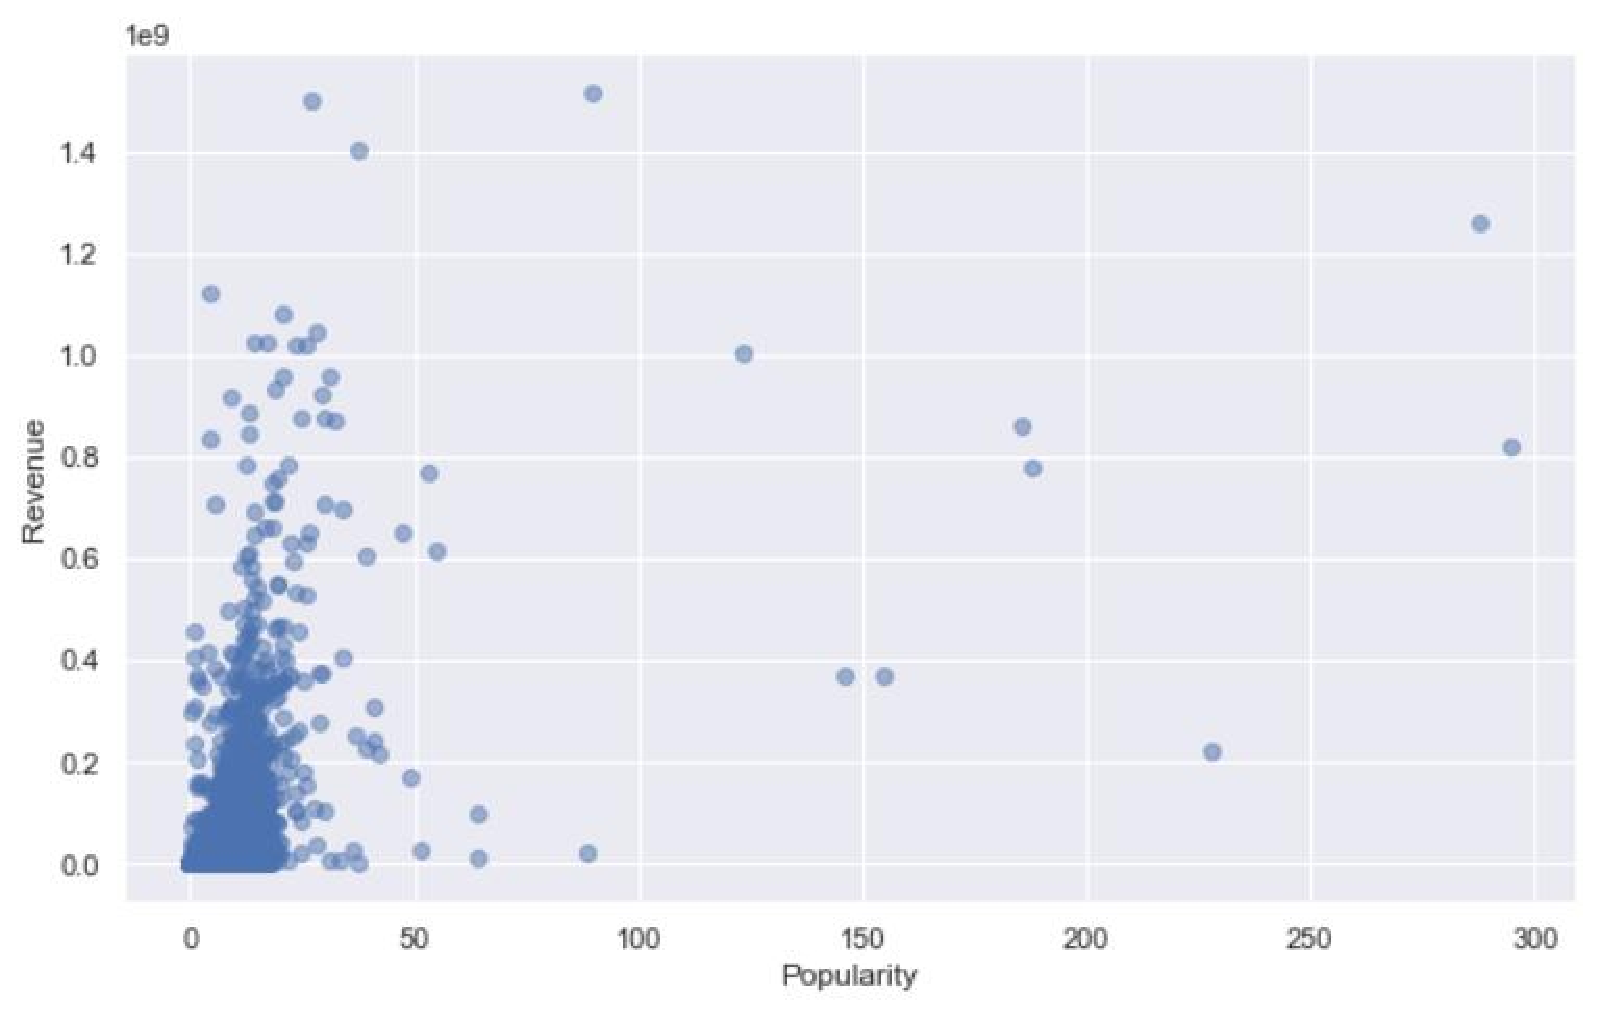
\includegraphics[scale=0.4]{./figures/popular2.eps}
  \caption{Popularity}
\end{figure}

\begin{figure}[htbp]
  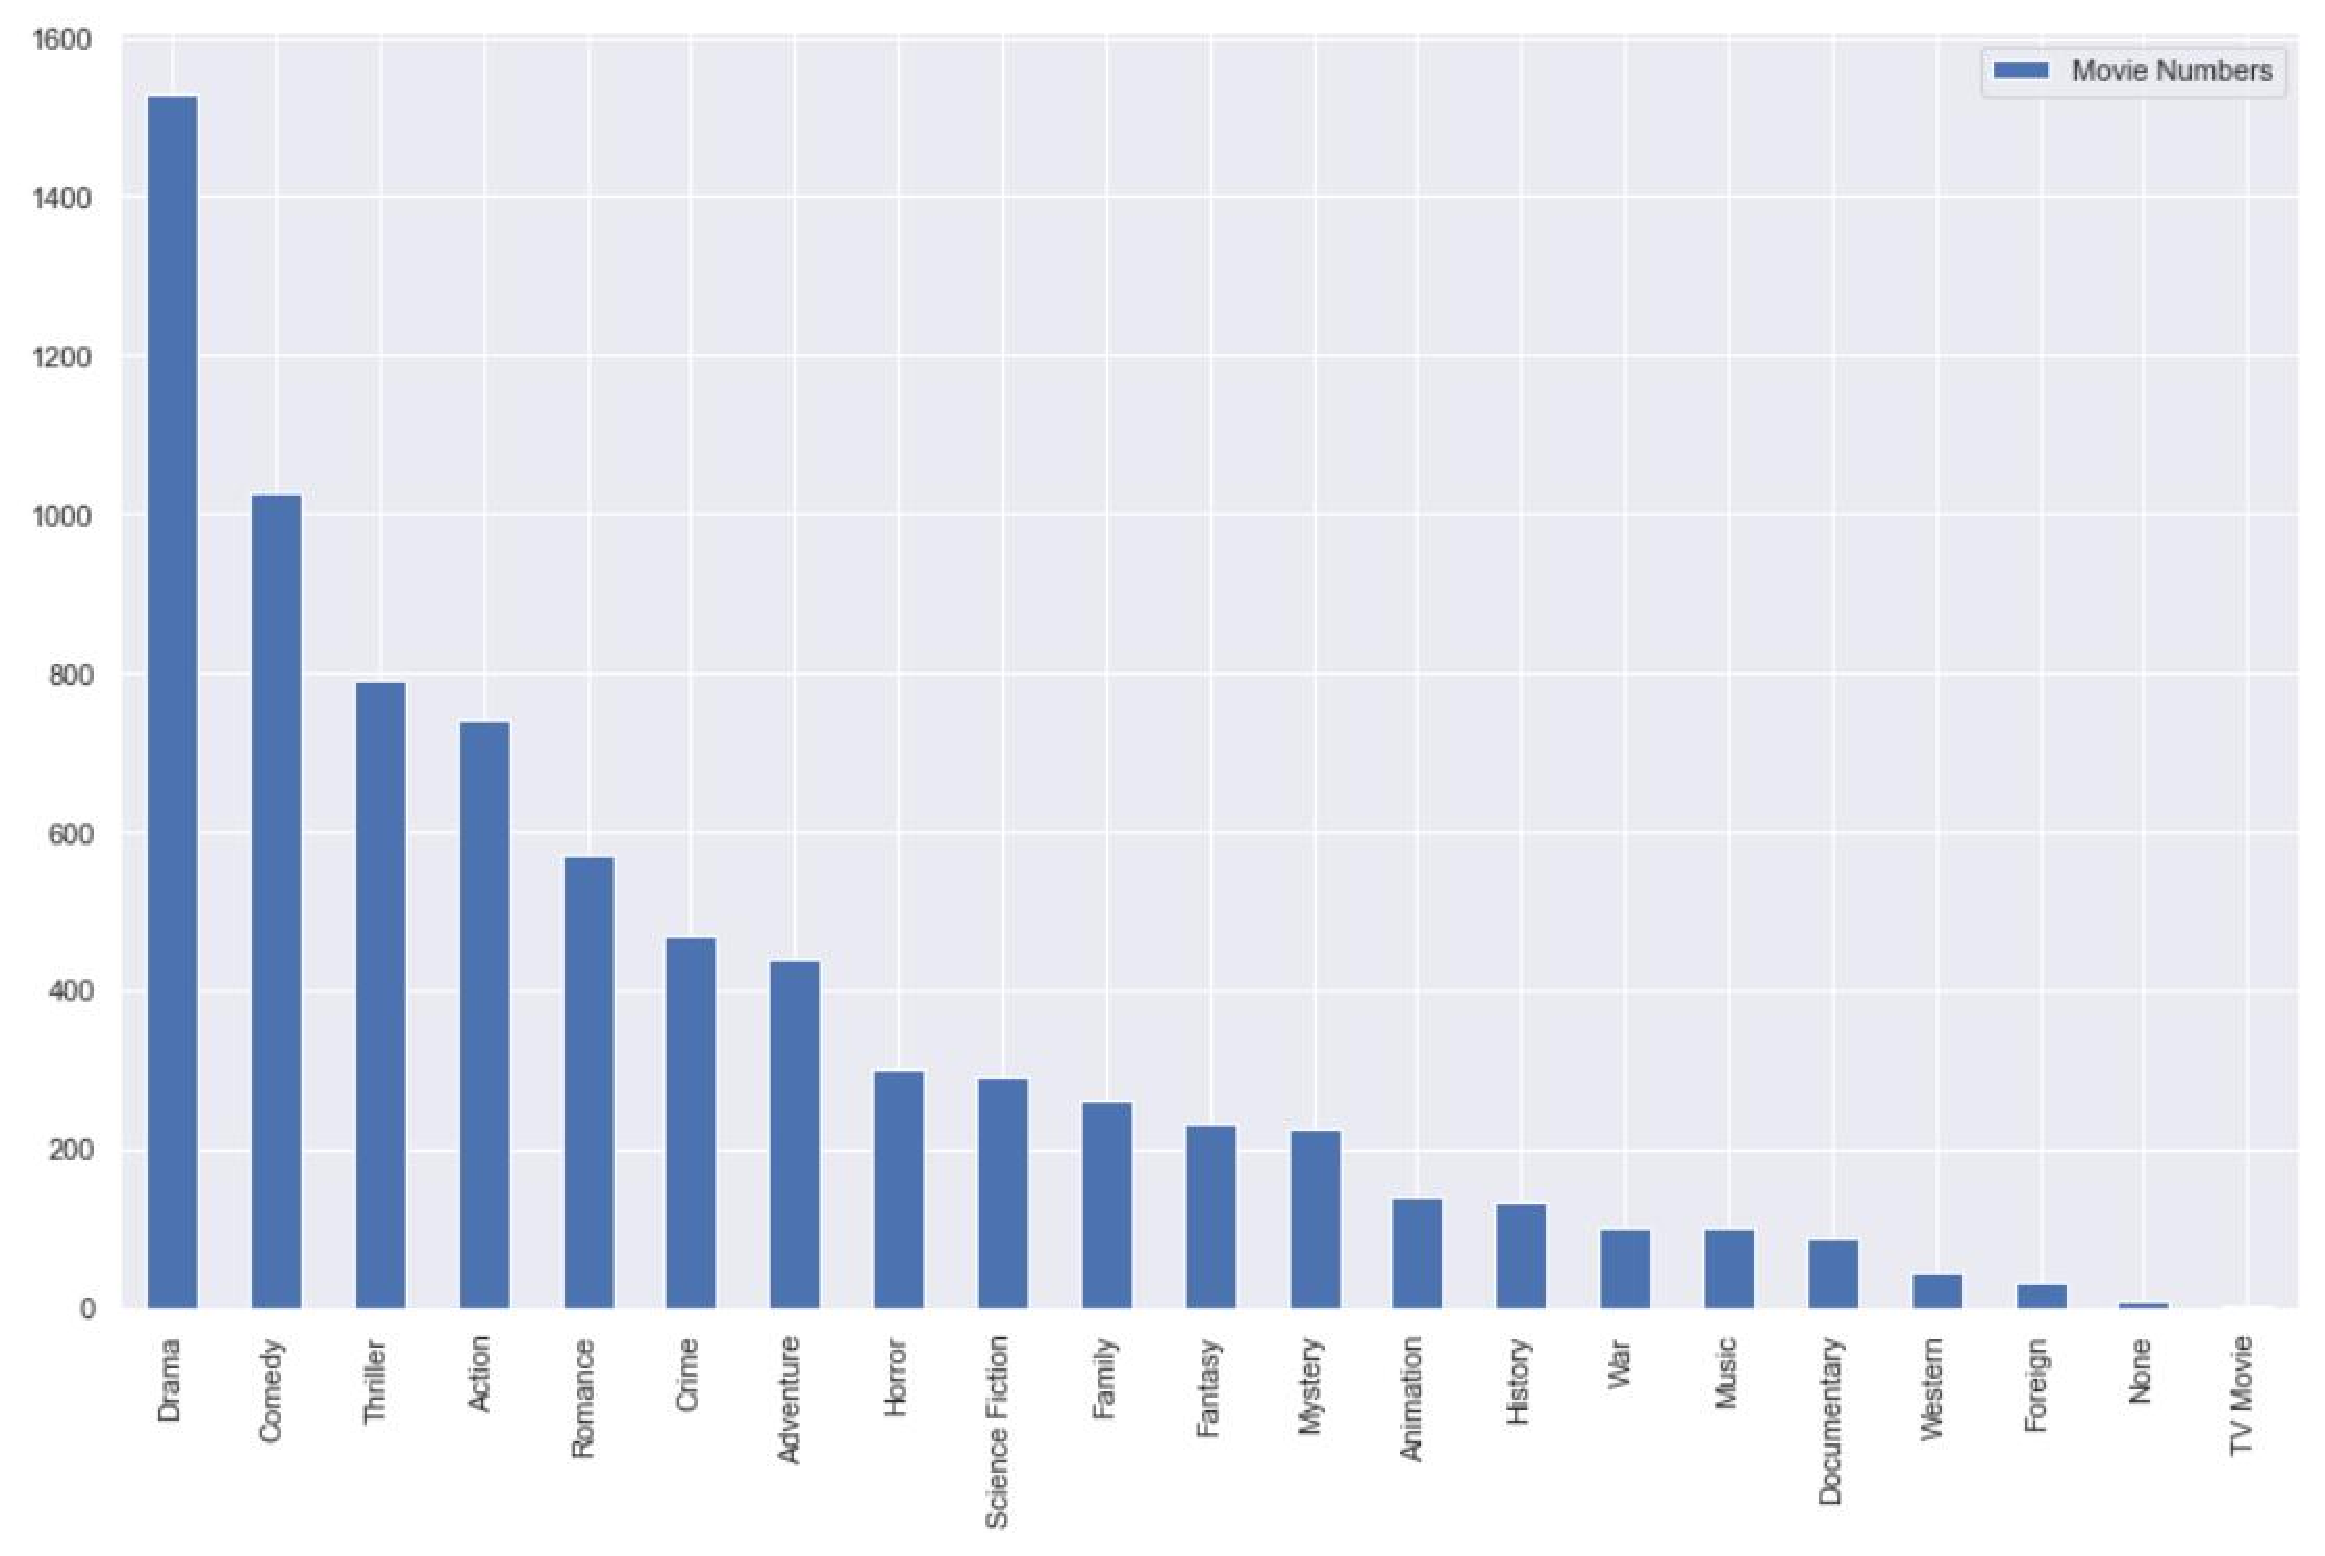
\includegraphics[width=0.9\textwidth,height=0.5\textwidth]{./figures/genres1.eps}
  \caption{Genres}
\end{figure}


\begin{figure}[htbp]
  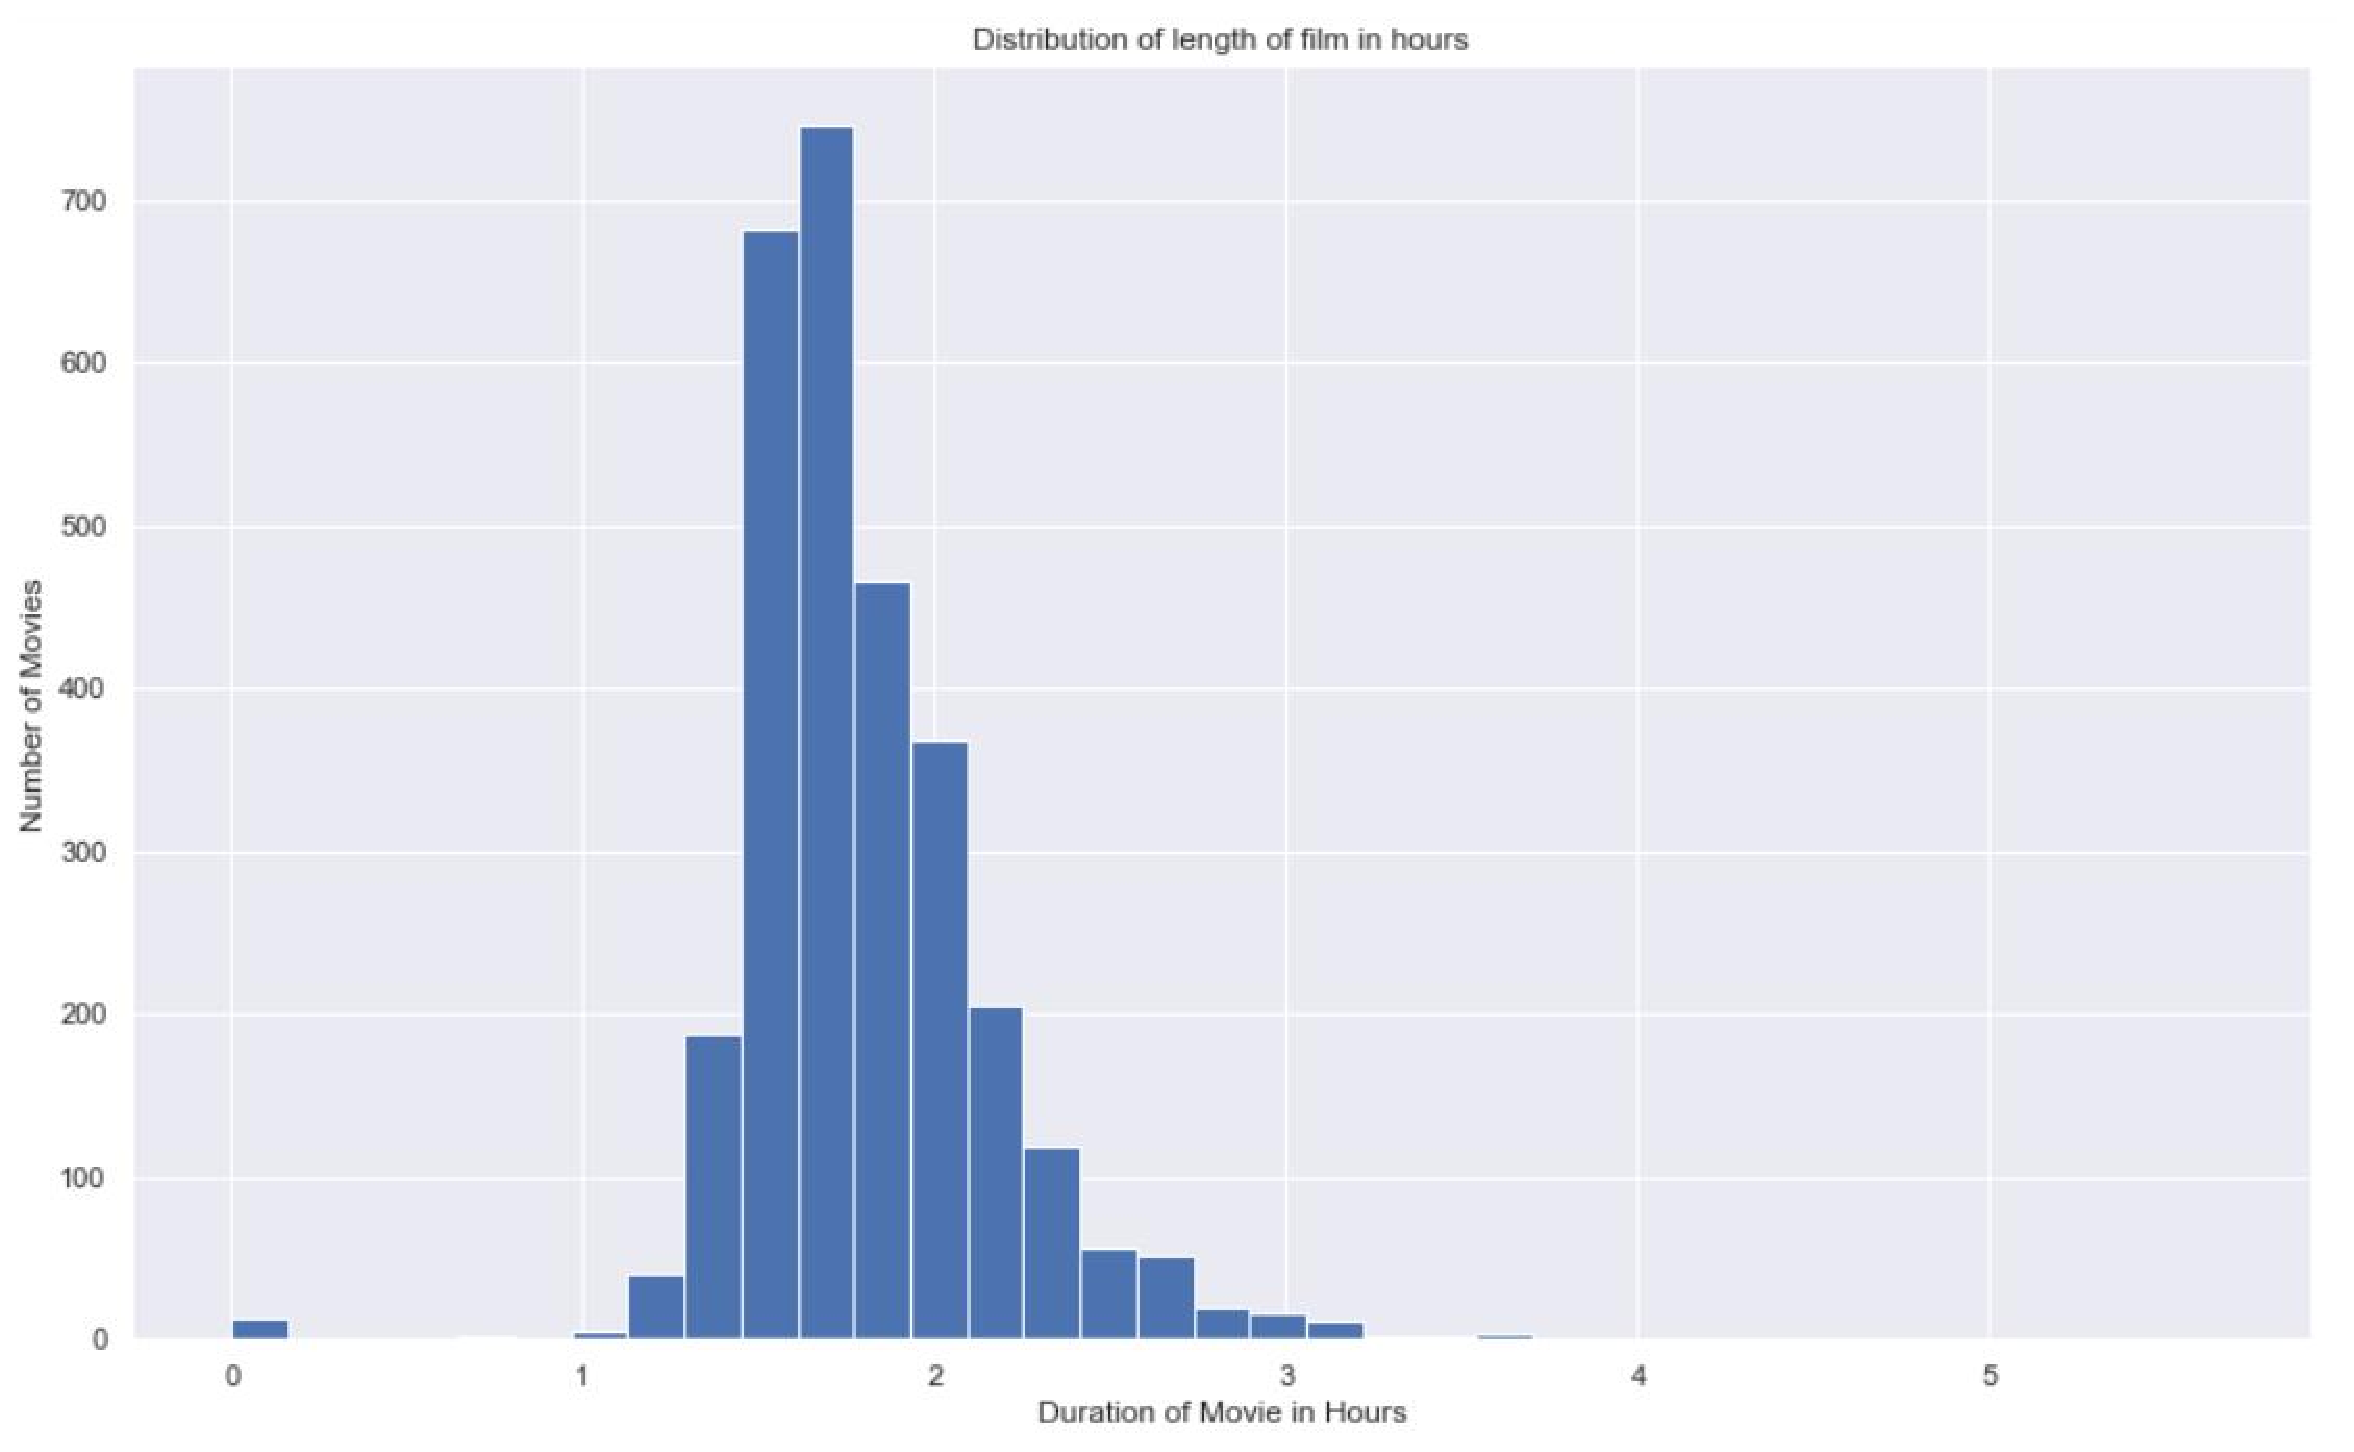
\includegraphics[width=0.9\textwidth,height=0.5\textwidth]{./figures/runtime1.eps}
  \caption{Runtime}
\end{figure}

\begin{figure}[htbp]
  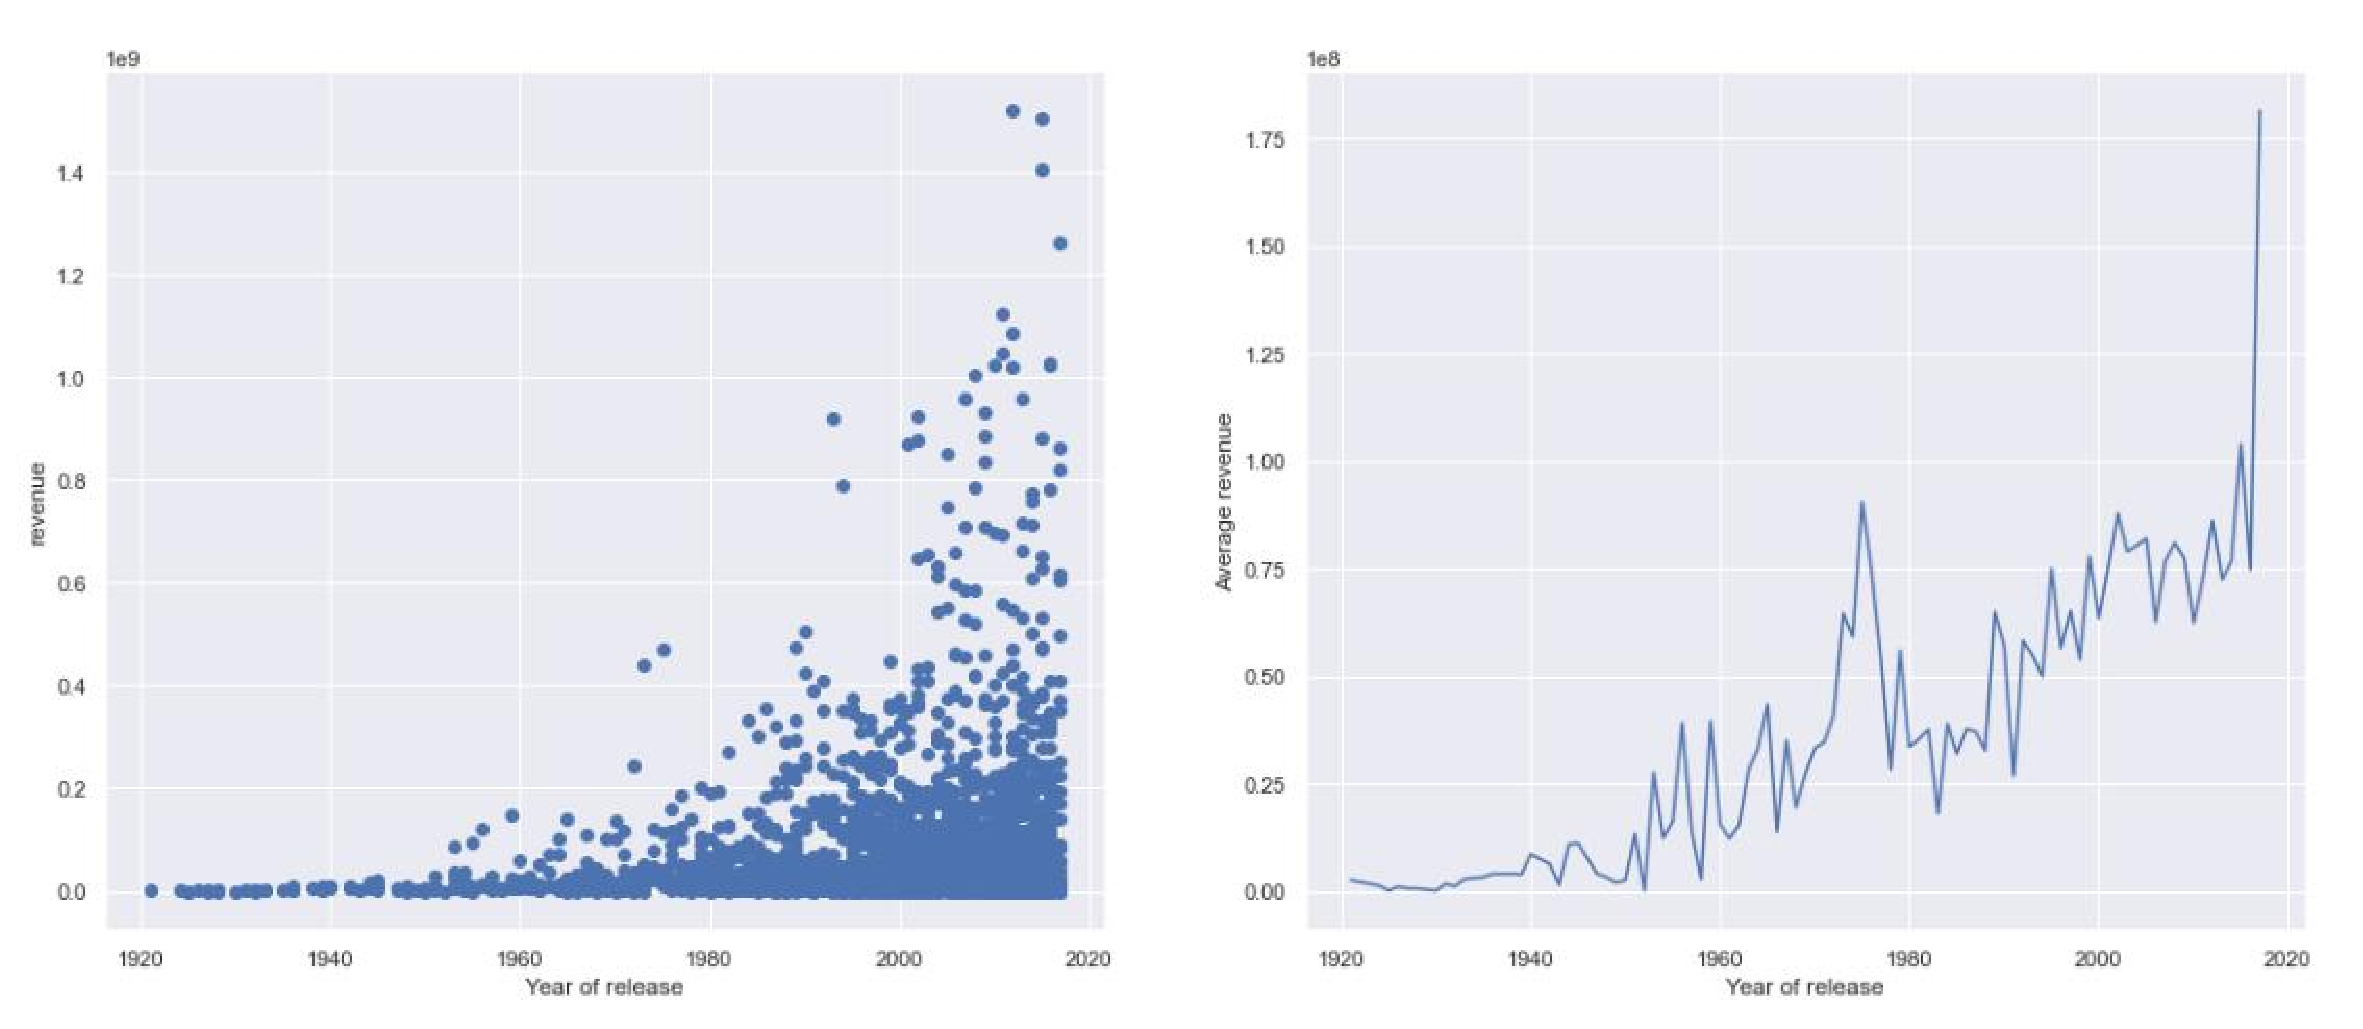
\includegraphics[width=0.9\textwidth,height=0.5\textwidth]{./figures/year2.eps}
  \caption{Date}
\end{figure}

Through correlation analysis of data visualization, we can find that there should be a positive correlation 
between budget and revenue, and the correlation between popularity and revenue should not be as strong as budget.
In addition, runtime and release dates should also have an impact on revenue.  \\


\section{Feature Selection And Model} \label{sec-preliminaries}
\subsection{Release date}
I selected a total of 9 dimensions, including release year, release month, release week, language, number of companies, 
number of crew, budget, popularity and Runtime.  \\

\subsection{Model and Result}
I used a random forest to train the data.A random forest is a classifier that contains multiple decision trees and whose output class is
determined by the plurality of the classes of the individual tree outputs.  \\
I use the root mean square error to measure the prediction gap.The root mean square error is the square root of the ratio of the deviation between the predicted
value and the true value to the number of observations n. In addition,I divided the data set into 0.8 training data set and 0.2 test data set. \\
Score:1.19 \\

\section{Conclusion} \label{sec-preliminaries}
The effect of the model is general, the main reason is that the selected features
are not comprehensive enough, and the learning and thinking of feature
selection should be strengthened in the future.

% ----------------------------------------------------------------
% \newpage
% \bibliography{tuliplab,yourbib}
% % TODO: you should change this yourbib into a proper bib file name
% \bibliographystyle{plainnat}
%=================================================================

%  \listoftodos

\end{document}

